\documentclass[11pt,a4paper]{article}
\usepackage{amsmath}
\usepackage{amssymb}
\usepackage{enumitem}
\usepackage{amsthm}
\usepackage{MnSymbol}
\setlength{\parindent}{0pt}
\usepackage[utf8]{inputenc}
\usepackage{listings} [python]
\usepackage{url}
\usepackage{bussproofs}
\usepackage{rotating}
\usepackage{tikz}
\usepackage{hyperref}

\newtheorem{theorem}{Theorem}[section]
\newtheorem{corollary}{Corollary}[theorem]
\newtheorem{lemma}[theorem]{Lemma}
\newtheorem{mydef}{Definition}

%opening


\newcommand{\lto}{\supset}
\newcommand{\some}{\Diamond}
\newcommand{\all}{\Box}

\newcommand{\tall}[1]{\left[ #1 \right]}
\newcommand{\tsome}[1]{\left\langle  #1 \right\rangle}

\newcommand{\eall}{\mathbf{K}}
\newcommand{\esome}{\mathbf{P}}
\newcommand{\edisp}{\mathbf{S}}
\newcommand{\edist}{\mathbf{D}}
\newcommand{\egen}{\mathbf{E}}
\newcommand{\ecom}{\mathbf{C}}

\newcommand{\sand}{\; and \;}
\newcommand{\sor}{ \; or \;}
\newcommand{\sneg}{not \;}
\newcommand{\sto}{\Rightarrow}
\newcommand{\negmodels}{\nvDash}


\newenvironment{changemargin}[2]{%
\begin{list}{}{%
\setlength{\topsep}{0pt}%
\setlength{\leftmargin}{#1}%
\setlength{\rightmargin}{#2}%
\setlength{\listparindent}{\parindent}%
\setlength{\itemindent}{\parindent}%
\setlength{\parsep}{\parskip}%
}%
\item[]}{\end{list}}

\begin{document}

%\maketitle


\section*{Exercise 44}
\begin{quote}
(Analogously to exercise 38:) Separate $\edist_G$ from $\eall_i$, $\edisp_G$, and $\edisp_G\edisp_G$ in a single connected model, if possible.
\end{quote}


Firstly, let $ab:=G=\{a,b\}$. Consider the following epistemic model $\mathcal{M}$.

\begin{center}
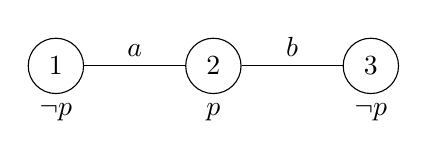
\begin{tikzpicture}
  \tikzset{vertex/.style = {shape=circle,draw,minimum size=2em,inner sep=1pt}}
  \tikzset{edge/.style = {->,- = latex'}}
	\node[vertex][label=below:$\neg p$] (1) at (0,0) {$1$};
	\node[vertex][label=below:$p$] (2) at (2,0) {$2$};
	\node[vertex][label=below:$\neg p$] (3) at (4,0) {$3$};


    \foreach \from/\to/\r in {1/2/a,2/3/b}
    \path[-](\from) edge node [above]{$\r$} (\to);
   
\end{tikzpicture}
\end{center}
\begin{enumerate}
\item $(\edist_G, \eall_a)$:\\
Consider state $2$. That is, $\mathcal{M},2 \nmodels \eall_a p$ due to $1$, and $\mathcal{M},2 \models \edist_G p$, because taking the intersection of $R_a$ and $R_b$ it follows that state $2$ is isolated. Hence all states accessible through $R_{D_G}$ satisfy $p$.

\item $(\edist_G, \eall_b)$:\\
Consider state $2$. That is, $\mathcal{M},2 \nmodels \eall_b p$ due to $3$, and $\mathcal{M},2 \models \edist_G p$, because taking the intersection of $R_a$ and $R_b$ it follows that state $2$ is isolated. Hence all states accessible through $R_{D_G}$ satisfy $p$.

\item $(\edist_G, \edisp_G)$:\\
Consider state $2$. That is, $\mathcal{M},2 \nmodels \edisp_G p$ due to $\mathcal{M},2 \models \eall_a p$  and $\mathcal{M},2 \models \eall_b p$. Moreover, $\mathcal{M},2 \models \edist_G p$, because taking the intersection of $R_a$ and $R_b$ it follows that state $2$ is isolated. Hence all states accessible through $R_{D_G}$ satisfy $p$.

\item $(\edist_G,  \edisp_G \edisp_G)$:\\
Consider state $2$. That is, $\mathcal{M},2 \nmodels \edisp_G p$, due to the fact that, as established above, $\mathcal{M},2 \nmodels \edisp_G p$  there exists at least one state accessible form $2$ via $R_a$ and via $R_b$ such that $\edisp_G p$ does not hold. Hence, $\mathcal{M},2 \nmodels  \eall_a \edisp_G p $ and $\mathcal{M},2 \nmodels \eall_b \edisp_G p$. Moreover, $\mathcal{M},2 \models \edist_G p$, because taking the intersection of $R_a$ and $R_b$ it follows that state $2$ is isolated. Hence all states accessible through $R_{D_G}$ satisfy $p$.
\end{enumerate}



\section*{Exercise 45}
\begin{quote}
Present a Kripke- and a Beth-countermodel for $\neg \neg A \lto A$.
\end{quote}
Before moving forward, an overview of the required definitions. 

\begin{mydef}
A model $\mathcal{M}:= \langle M, \leqslant , D, \Vdash \rangle$.
\begin{itemize}
\item $(M, \leqslant)$ is a partially ordered set.
\item $D$ assigns a structure to $\gamma \in M$, s.t. $\alpha, \beta \in M \; \alpha \leqslant \beta \sto D(\alpha) \subseteq D(\beta)$. (subset relation)
\item $\Vdash \subseteq M \times M$.
\begin{enumerate}
\item $\alpha \Vdash p$, if there is a bar $B$ for $\alpha$, s.t. $\forall \beta \in B$, $D(\beta) \models p$;
\item $\alpha \Vdash \varphi \land \psi$, if $\alpha \Vdash \varphi \sand \alpha \Vdash  \psi$;
\item $\alpha \Vdash \varphi \lor \psi$,  if there is a bar $B$ for $\alpha$, s.t. $\forall \beta \in B (\beta  \Vdash  \varphi \sor \beta  \Vdash  \psi)$;
\item $\alpha \Vdash \varphi \lto \psi$, if $\forall \beta \geqslant \alpha (\beta \Vdash \varphi \sto \beta \Vdash \psi)$;
\item $\alpha \Vdash \forall x\; \varphi(x)$, if $\forall \beta \geqslant \alpha (\forall b \in |D(\beta)| \; \beta \Vdash \varphi(b))$;
\item $\alpha \Vdash \exists x\; \varphi(x)$, if there is a bar $B$ for $\alpha$, s.t. $\forall \beta \in B (\exists b \in |D(\beta)| \; \beta \Vdash \varphi(b))$;
\item $\alpha \Vdash \neg \varphi$, if $\forall \beta \geqslant \alpha (\beta \nVdash \varphi)$.
\end{enumerate}
\end{itemize}
\end{mydef}

Moreover, 

\begin{mydef}
A formula $\varphi$ holds in a model $\mathcal{M}$ if $\alpha \Vdash cl(\varphi)$ for all $\alpha$, where $cl(\varphi)$ is the universal closure of $\varphi$.
\end{mydef}

Furthermore, a nice lemma was also presented.

\begin{lemma}
The following statements hold:
\begin{enumerate}
\item For $\alpha \leqslant \beta$, $\alpha \Vdash \varphi \sto \beta \Vdash \varphi$;
\item For $\alpha \nVdash \varphi \Leftrightarrow$ there is a path $P$ through $\alpha$ such that $\forall \beta \in P (\beta \nVdash \varphi)$;
\item For $\alpha \Vdash \varphi \Leftrightarrow$ there is a bar $B$ for $\alpha$ such that $\forall \beta \in B (\beta \Vdash \varphi)$;
\end{enumerate}
\end{lemma}


Moreover, the definition for a Beth model
\begin{mydef}
$\mathcal{M}$ is a Beth model if $|D(\alpha)|$ is a fixed set $D$ for all $\alpha$. 
\begin{enumerate}
\item $\alpha \Vdash p$, if there is a bar $B$ for $\alpha$, s.t. $\forall \beta \in B$, $D(\beta) \models p$;
\item $\alpha \Vdash \varphi \land \psi$, if $\alpha \Vdash \varphi \sand \alpha \Vdash  \psi$;
\item $\alpha \Vdash \varphi \lor \psi$,  if there is a bar $B$ for $\alpha$, s.t. $\forall \beta \in B (\beta  \Vdash  \varphi \sor \beta  \Vdash  \psi)$;
\item $\alpha \Vdash \varphi \lto \psi$, if $\forall \beta \geqslant \alpha (\beta \Vdash \varphi \sto \beta \Vdash \psi)$;
\item $\alpha \Vdash \forall x \varphi(x) \Leftrightarrow \forall a \in D (\alpha \Vdash \varphi(a))$
\item $\alpha \Vdash \exists x\; \varphi(x)$, if there is a bar $B$ for $\alpha$, s.t. $\forall \beta \in B (\exists b \in |D(\beta)| \; \beta \Vdash \varphi(b))$;
\item $\alpha \Vdash \neg \varphi$, if $\forall \beta \geqslant \alpha (\beta \nVdash \varphi)$.
\end{enumerate}
\end{mydef}

and a Kripke model is defined as 
\begin{mydef}
$\mathcal{M}$ is a Kripke model if in (1), (3) and (6), $B=\{a\}$, i.e.
\begin{enumerate}
\item $\alpha \Vdash p$, if $D(\alpha) \models p$;
\item $\alpha \Vdash \varphi \land \psi$, if $\alpha \Vdash \varphi \sand \alpha \Vdash  \psi$;
\item $\alpha \Vdash \varphi \lor \psi$, if $\alpha  \Vdash  \varphi \sor \alpha  \Vdash  \psi$;
\item $\alpha \Vdash \varphi \lto \psi$, if $\forall \beta \geqslant \alpha (\beta \Vdash \varphi \sto \beta \Vdash \psi)$;
\item $\alpha \Vdash \forall x\; \varphi(x)$, if $\forall \beta \geqslant \alpha (\forall b \in |D(\beta)| \; \beta \Vdash \varphi(b))$;
\item $\alpha \Vdash \exists x\; \varphi(x)$, if $\exists a \in |D(\alpha)| \; \alpha \Vdash \varphi(a)$;
\item $\alpha \Vdash \neg \varphi$, if $\forall \beta \geqslant \alpha (\beta \nVdash \varphi)$.
\end{enumerate}
\end{mydef}


Starting with the semantic unravelling of the sentence $\neg \neg \varphi \lto \varphi$.
\begin{align*}
&\alpha \Vdash \neg \neg \varphi \lto \varphi   && \iff & \\
&\forall \beta \geqslant \alpha (\beta \Vdash \neg \neg \varphi \sto  \beta \Vdash \varphi )  && \iff & \\
&\forall \beta \geqslant \alpha ( \forall \gamma \geqslant \beta (\sneg \gamma \Vdash \neg \varphi) \sto  \beta \Vdash \varphi )  && \iff & \\
&\forall \beta \geqslant \alpha ( \forall \gamma \geqslant \beta (\sneg (\forall \delta \geqslant \gamma \; \sneg \delta \Vdash \varphi )) \sto  \beta \Vdash \varphi )  && \iff & \\
&\forall \beta \geqslant \alpha ( \forall \gamma \geqslant \beta (\exists \delta \geqslant \gamma \; \delta \Vdash  \varphi ) \sto  \beta \Vdash \varphi )  && \iff & \\
\end{align*}

Firstly, consider the following Kripke model.
\begin{center}
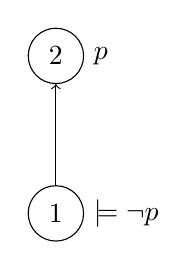
\begin{tikzpicture}
  \tikzset{vertex/.style = {shape=circle,draw,minimum size=2em,inner sep=1pt}}
  \tikzset{edge/.style = {->,- = latex'}}
	\node[vertex][label=right :$\models \neg p$] (1) at (0,0) {$1$};
	\node[vertex][label=right:$p$] (2) at (0,2) {$2$};

	
    \foreach \from/\to in {1/2}
    \path[->](\from) edge node [above]{} (\to);
\end{tikzpicture}
\end{center}
where $|D(1)|=|D(2)|= \{a\}$ and $p$ is a predicate of arity $0$.
First, one has to confirm that this model actually satisfies the required properties. Clearly, the set of worlds is a partial order (reflexive edges are not drawn).
Since $1 \leqslant 2$ and $D(1) \nmodels p$ and  $D(2) \models p$, it is the case that $D(1) \subseteq D(2)$. Hence, given
\begin{equation*}
\forall \beta \geqslant \alpha ( \forall \gamma \geqslant \beta (\exists \delta \geqslant \gamma \; \delta \Vdash  p ) \sto  \beta \Vdash p ) 
\end{equation*}
and the fact that this is a Kripke model it follows
\begin{equation*}
\forall \beta \geqslant \alpha ( \forall \gamma \geqslant \beta (\exists \delta \geqslant \gamma \; D(\delta) \models  p ) \sto  D(\beta) \models p ) 
\end{equation*}
Now consider $1$ as $\alpha$  and $1$ as $\beta$, by reflexivity $1 \geqslant 1$, resulting in 
\begin{equation*}
 \forall \gamma \geqslant 1 (\exists \delta \geqslant \gamma \; D(\delta) \models  p ) \sto  D(1) \models p 
\end{equation*}
Clearly $ D(1) \models p $ can not be the case. Hence, if the premise is correct $\mathcal{M}$ is a counter model. To establish exactly that two case distinctions are required.
\begin{itemize}
\item \emph{Case 1:} For $\gamma$ is $1$, we have $2 \geqslant 1$ such that $D(2) \models p$.
\item \emph{Case 2:} For $\gamma$ is $2$, we have $2\geqslant 2$ such that $D(2) \models p$.
\end{itemize}
Hence, the premise of the implication is satisfied by $\mathcal{M}$, thus a counter Kripke model is found.

Secondly, consider the following Beth model $\mathcal{M}:= \langle  M , \leqslant, D, \Vdash \rangle$. Where $M:=M_o \cup M_p=\{\underline{1},\underline{2},\underline{3} \dots\}\cup \{\underline{1}_p,\underline{2}_p,\underline{3}_p,\dots\}$ and $\leqslant$ is the reflexive, anti-symmetric and transitive closure of $\{(\underline{1},\underline{1}_p), (\underline{1},\underline{2}), (\underline{2},\underline{2}_p), (\underline{2},\underline{3}), (\underline{3},\underline{3}_p) ,\dots\}$, as well as $\forall \alpha \in M_o \; D(\alpha)\nmodels p$ and $\forall \alpha \in M_p \; D(\alpha)\models p$.
The following is a visualisation for the first three steps.
\begin{center}
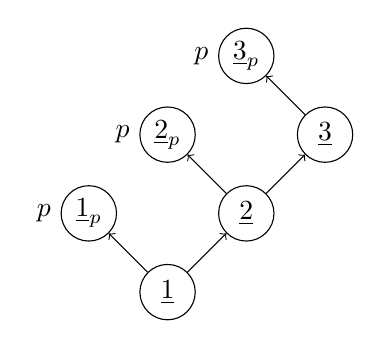
\begin{tikzpicture}
  \tikzset{vertex/.style = {shape=circle,draw,minimum size=2em,inner sep=1pt}}
  \tikzset{edge/.style = {->,- = latex'}}
	\node[vertex](1) at (1,0) {$\underline{1}$};
	\node[vertex][label=left:$p$] (1p) at (0,1) {$\underline{1}_p$};

	\node[vertex](2) at (2,1) {$\underline{2}$};
	\node[vertex][label=left:$p$] (2p) at (1,2) {$\underline{2}_p$};
	
		\node[vertex](3) at (3,2) {$\underline{3}$};
	\node[vertex][label=left:$p$] (3p) at (2,3) {$\underline{3}_p$};

	
    \foreach \from/\to in {1/1p,2/2p,3/3p, 1/2,2/3}
    \path[->](\from) edge node [above]{} (\to);
\end{tikzpicture}
\end{center}

First, one has to confirm that this model actually satisfies the required properties. Clearly, the set of worlds is a partial order (reflexive and transitive edges are not drawn). 
Moreover, $\forall \alpha |D(\alpha)|=\{\}$, since only propositional statements are considered.
For any arbitrary $k >0$ it follows that, $\underline{k}\leqslant \underline{k}_p$ and $D(\underline{k}) \nmodels p$ and  $D(\underline{k}_p) \models p$, it is the case that $D(\underline{k}) \subseteq D(\underline{k}_p)$. Similarly, since $ \underline{k} \leqslant \underline{k+1}$ and $D( \underline{k}) \nmodels p$ and  $D( \underline{k+1}) \nmodels p$, it is the case that $D( \underline{k}) \subseteq D( \underline{k+1})$. Hence, given
\begin{equation*}
\forall \beta \geqslant \alpha ( \forall \gamma \geqslant \beta (\exists \delta \geqslant \gamma \; \delta \Vdash  p ) \sto  \beta \Vdash p ) 
\end{equation*}
and the fact that this is a Beth model it follows
\begin{equation*}
\forall \beta \geqslant \alpha ( \forall \gamma \geqslant \beta (\exists \delta \geqslant \gamma \; \exists \mathcal{B}_{\delta}\forall \epsilon \in  \mathcal{B}_{\delta} \; D(\epsilon) \models p) \sto  \exists \mathcal{B}_{\beta}\forall \gamma \in  \mathcal{B}_{\beta} \; D(\gamma) \models p) 
\end{equation*}
Where $\exists \mathcal{B}_{\alpha}\forall \beta \in  \mathcal{B}_{\alpha} \; D(\beta) \models p$ is a shorthand for  "if there is a bar $B$ for $\alpha$, s.t. $\forall \beta \in B$, $D(\beta) \models p$".\\

Now consider $ \underline{1}$ as $\alpha$. The statement $ \exists \mathcal{B}_{\beta}\forall \gamma \in  \mathcal{B}_{\beta} \; D(\gamma) \models p$ can not hold due to the fact that it would require that at some point there exists a bar, such that for all states in the bar it follows that $p$ holds. However, with $M_o$ being infinite and $ \underline{1} \leqslant  \underline{k}$ for $ \underline{k} \in M_o$ such bar can not exist. That is, at every point of the path $ \underline{1}, \underline{2},\dots, \underline{k}$ we know that $p$ can not hold. Moreover, it is possible to find an path of arbitrary length of that kind. Hence, for any given bar, there exists a path of that kind that intersects with this bar. Thereby, invalidating the statement  $\exists \mathcal{B}_{\beta}\forall \gamma \in  \mathcal{B}_{\beta} \; D(\gamma) \models p$. \\

Hence, if the premise is correct $\mathcal{M}$ is a counter model. To establish exactly that, two case distinctions are required.
Consider an arbitrary $k \geqslant 1$
\begin{itemize}
\item \emph{Case 1:} For $\gamma$ is $\underline{k}$, we have $\underline{k}_p$ as $\delta$ due to $\underline{k}_p \geqslant \underline{k}$ such that $D(\underline{k}_p) \models p$. In this case $ \mathcal{B}_{\delta}=  \mathcal{B}_{\underline{k}_b}=\{\underline{k}_b\}$.
\item \emph{Case 2:} For $\gamma$ is $\underline{k}_p$, we have $\underline{k}_p$ as $\delta$ due to $\underline{k}_p \geqslant \underline{k}_p$ such that $D(\underline{k}_p) \models p$. In this case $ \mathcal{B}_{\delta}=  \mathcal{B}_{\underline{k}_b}=\{\underline{k}_b\}$.

\end{itemize}
Hence, the premise of the implication is satisfied by $\mathcal{M}$, thus a counter Beth model is found.


\section*{Exercise 46}
\begin{quote}
Present a Kripke-countermodel for $\neg \forall x \neg P(x) \lto \exists x P(x)$.
\end{quote}



Starting with the semantic unravelling of the sentence $\neg \forall x \neg P(x) \lto \exists x P(x)$ with respect to a Kripke model.

\begin{changemargin}{-1cm}{-1cm}
\begin{align*}
&\neg \forall x \neg P(x) \lto \exists x P(x)   & \\
&\forall \beta \geqslant \alpha (\beta \Vdash \neg \forall x \neg P(x) \sto  \beta \Vdash \exists x P(x) )  & \\
&\forall \beta \geqslant \alpha (\forall \gamma \geqslant \beta (\sneg  \gamma \Vdash  \forall x \neg P(x)) \sto  \beta \Vdash \exists x P(x) )  & \\
&\forall \beta \geqslant \alpha (\forall \gamma \geqslant \beta (\sneg   \forall \delta \geqslant \gamma  \forall x_{\delta} \in |D(\delta)| (\delta \Vdash  \neg P(x_{\delta}))) \sto  \beta \Vdash \exists x P(x) )  &\\
&\forall \beta \geqslant \alpha (\forall \gamma \geqslant \beta (\sneg   \forall \delta \geqslant \gamma  \forall x_{\delta} \in |D(\delta)| (\forall \epsilon \geqslant \delta (\sneg  D(\epsilon) \models P(x_{\delta})))) \sto  \beta \Vdash \exists x P(x) )  &\\
&\forall \beta \geqslant \alpha (\forall \gamma \geqslant \beta (\sneg   \forall \delta \geqslant \gamma  \forall x_{\delta} \in |D(\delta)| (\forall \epsilon \geqslant \delta (\sneg  D(\epsilon) \models P(x_{\delta})))) \sto \exists x_{\beta} \in |D( \beta)| (D(\beta) \models P(x_{\beta}) ))  & \\
&\forall \beta \geqslant \alpha (\forall \gamma \geqslant \beta ( \exists \delta \geqslant \gamma  \exists x_{\delta} \in |D(\delta)| (\exists \epsilon \geqslant \delta ( D(\epsilon) \models P(x_{\delta})))) \sto \exists x_{\beta} \in |D( \beta)| (D(\beta) \models P(x_{\beta}) ))  & \\
\end{align*}
\end{changemargin}

Consider the following Kripke model $\mathcal{M}$.
\begin{center}
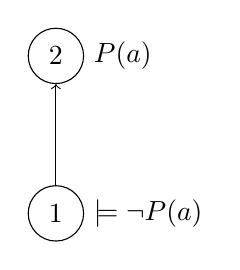
\begin{tikzpicture}
  \tikzset{vertex/.style = {shape=circle,draw,minimum size=2em,inner sep=1pt}}
  \tikzset{edge/.style = {->,- = latex'}}
	\node[vertex][label=right :$\models \neg P(a)$] (1) at (0,0) {$1$};
	\node[vertex][label=right:$P(a)$] (2) at (0,2) {$2$};

    \foreach \from/\to in {1/2}
    \path[->](\from) edge node [above]{} (\to);
\end{tikzpicture}
\end{center}
where $|D(1)|=|D(2)|=\{a\}$ and $D(1)\nmodels P(a)$ while $D(2)\models P(a)$.

First, one has to confirm that this model actually satisfies the required properties. Clearly, the set of worlds is a partial order (reflexive edges are not drawn).
Since $1 \leqslant 2$ and $D(1) \nmodels P(a)$ and  $D(2) \models P(a)$, it is the case that $D(1) \subseteq D(2)$. 

Now consider $1$ as $\alpha$  and $1$ as $\beta$, by reflexivity $1 \geqslant 1$, resulting in 
\begin{equation*}
\forall \gamma \geqslant \beta ( \exists \delta \geqslant \gamma  \exists x_{\delta} \in |D(\delta)| (\exists \epsilon \geqslant \delta ( D(\epsilon) \models P(x_{\delta})))) \sto \exists x_{\beta} \in |D( \beta)| (D(\beta) \models P(x_{\beta}) )
\end{equation*}
With $a$ being the only element in the domain and with $ D(1) \nmodels P(a)$ it follows that $ \exists x_{1} \in |D( 1)| \; D(1) \models P(x_1) $ can not hold. Hence, if the premise is correct $\mathcal{M}$ is a counter model. To establish exactly that two case distinctions are required.
\begin{itemize}
\item \emph{Case 1:} For $\gamma$ is $1$, we have $2 \geqslant 1$ for $\delta$ and $2 \geqslant 2$ for $\epsilon$ such that $D(2) \models P(a)$.
\item \emph{Case 2:} For $\gamma$ is $2$, we have $2 \geqslant 2$ for $\delta$ and $2 \geqslant 2$ for $\epsilon$ such that $D(2) \models P(a)$.
\end{itemize}
Hence, the premise of the implication is satisfied by $\mathcal{M}$, thus a counter Kripke model is found.

\section*{Exercise 47}
\begin{quote}
Consider the classical laws of distribution ($\lor$ over $\land$, $\land$ over $\lor$). Which parts of these laws (implications) hold and which fail
for intuitionistic logic?
Provide sequent or natural deduction proofs for the positive cases and Kripke and/or Beth counterexamples for the negative cases.
\end{quote}

As far as I am aware the laws in question are:
\begin{enumerate}
\item $(P\land (Q\lor R))\lto ((P\land Q)\lor (P\land R))$
\item $(P\lor (Q\land R))\lto ((P\lor Q)\land (P\lor R))$
\item $((P\land Q)\lor (P\land R)) \lto  (P\land (Q\lor R)) $
\item $((P\lor Q)\land (P\lor R)) \lto (P\lor (Q\land R)) $
\end{enumerate}

Note that the inference 
\begin{prooftree}
\def\fCenter{\ \vdash\ }
\Axiom$\Gamma, \psi , \chi \fCenter \varphi$
\UnaryInf$\Gamma ,\psi \land \chi \fCenter \varphi$
\end{prooftree}
is a short cut for 
\begin{prooftree}
\def\fCenter{\ \vdash\ }
\Axiom$\Gamma, \psi , \chi \fCenter \varphi$
\UnaryInf$\Gamma ,\psi  ,\psi \land \chi \fCenter \varphi$
\UnaryInf$\Gamma ,\psi \land \chi ,\psi \land \chi \fCenter \varphi$
\UnaryInf$\Gamma ,\psi \land \chi \fCenter \varphi$
\end{prooftree}

For $(P\land (Q\lor R))\lto ((P\land Q)\lor (P\land R))$ the sequent proof is
\begin{prooftree}
\def\fCenter{\ \vdash\ }

		\AxiomC{}
		\UnaryInf$P \fCenter P$
		\UnaryInf$P, Q \fCenter P$

		\AxiomC{}
		\UnaryInf$Q \fCenter Q$
		\UnaryInf$P, Q \fCenter Q$

	\BinaryInf$P, Q \fCenter P\land Q$
	\UnaryInf$P, Q \fCenter (P\land Q)\lor (P\land R)$

		\AxiomC{}
		\UnaryInf$P \fCenter P$
		\UnaryInf$P, R \fCenter P$

		\AxiomC{}
		\UnaryInf$R \fCenter R$
		\UnaryInf$P, R \fCenter R$

	\BinaryInf$P, R \fCenter P\land R$
	\UnaryInf$P, R \fCenter (P\land Q)\lor (P\land R)$


\BinaryInf$P, (Q\lor R) \fCenter (P\land Q)\lor (P\land R)$
\UnaryInf$P\land (Q\lor R) \fCenter (P\land Q)\lor (P\land R)$
\UnaryInf$\fCenter (P\land (Q\lor R))\lto ((P\land Q)\lor (P\land R))$
\end{prooftree}



For $(P\lor (Q\land R))\lto ((P\lor Q)\land (P\lor R))$ the sequent proof is
\begin{prooftree}
\def\fCenter{\ \vdash\ }

			\AxiomC{}
			\UnaryInf$P \fCenter P$
			\UnaryInf$P \fCenter P\lor Q$

			\AxiomC{}
			\UnaryInf$P \fCenter P$
			\UnaryInf$P \fCenter P\lor R$
			
		\BinaryInf$P \fCenter (P\lor Q)\land (P\lor R)$
		
		
			\AxiomC{}
			\UnaryInf$Q \fCenter Q$
			\UnaryInf$Q, R \fCenter  Q$
			\UnaryInf$Q, R \fCenter P\lor Q$
			\AxiomC{}
			\UnaryInf$R \fCenter  R$
			\UnaryInf$Q, R \fCenter  R$
			\UnaryInf$Q, R \fCenter P\lor R$
		\BinaryInf$Q, R \fCenter (P\lor Q)\land (P\lor R)$
		\UnaryInf$Q\land R \fCenter (P\lor Q)\land (P\lor R)$
		
\BinaryInf$P\lor (Q\land R) \fCenter (P\lor Q)\land (P\lor R)$
\UnaryInf$\fCenter (P\lor (Q\land R))\lto ((P\lor Q)\land (P\lor R))$
\end{prooftree}


For $((P\land Q)\lor (P\land R)) \lto  (P\land (Q\lor R)) $ the sequent proof is
\begin{prooftree}
\def\fCenter{\ \vdash\ }

			\AxiomC{}
			\UnaryInf$P \fCenter  P$
			\UnaryInf$P, Q \fCenter P$
			
			\AxiomC{}
			\UnaryInf$Q \fCenter  Q$
			\UnaryInf$P, Q \fCenter Q$
			\UnaryInf$P, Q \fCenter Q\lor R$
			
		\BinaryInf$P, Q \fCenter P\land (Q\lor R)$
		\UnaryInf$P\land Q \fCenter P\land (Q\lor R)$
		
			\AxiomC{}
			\UnaryInf$P \fCenter  P$
			\UnaryInf$P, R \fCenter P$
			
			\AxiomC{}
			\UnaryInf$R \fCenter  R$
			\UnaryInf$P, R \fCenter R$
			\UnaryInf$P, R \fCenter Q\lor R$
		\BinaryInf$P, R \fCenter P\land (Q\lor R)$
		\UnaryInf$P\land R \fCenter P\land (Q\lor R)$
		
\BinaryInf$(P\land Q)\lor (P\land R) \fCenter P\land (Q\lor R)$
\UnaryInf$\fCenter ((P\land Q)\lor (P\land R)) \lto  (P\land (Q\lor R))$
\end{prooftree}



For $((P\lor Q)\land (P\lor R)) \lto (P\lor (Q\land R)) $ the sequent proof is
\begin{prooftree}
\scriptsize
\def\fCenter{\ \vdash\ }

			\AxiomC{}
			\UnaryInf$P\fCenter P$
			\UnaryInf$P, P \fCenter P$
			\UnaryInf$P, P \fCenter P\lor (Q\land R)$
			
			\AxiomC{}
			\UnaryInf$P \fCenter P$
			\UnaryInf$P, R \fCenter P$
			\UnaryInf$P, R \fCenter P\lor (Q\land R)$
			\BinaryInf$P, (P\lor R) \fCenter P\lor (Q\land R)$
			
			\AxiomC{}
			\UnaryInf$P \fCenter P$
			\UnaryInf$Q, P \fCenter P$
			\UnaryInf$Q, P \fCenter P\lor (Q\land R)$
			
				\AxiomC{}
				\UnaryInf$Q \fCenter Q$
				\UnaryInf$Q, R \fCenter Q$
								
				\AxiomC{}
				\UnaryInf$R \fCenter R$
				\UnaryInf$Q, R \fCenter R$
			\BinaryInf$Q, R \fCenter (Q\land R)$
			\UnaryInf$Q, R \fCenter P\lor (Q\land R)$
			\BinaryInf$Q, (P\lor R) \fCenter P\lor (Q\land R)$
		
\BinaryInf$(P\lor Q), (P\lor R) \fCenter P\lor (Q\land R)$
\UnaryInf$(P\lor Q)\land (P\lor R) \fCenter P\lor (Q\land R)$
\UnaryInf$\fCenter ((P\lor Q)\land (P\lor R)) \lto (P\lor (Q\land R))$
\end{prooftree}


%\section*{Exercise 37}
%\begin{quote}
%\begin{theorem}
%Multi-(n)-modal \textbf{S5} is the smallest normal modal logic, based on frames with accessibility relations $R_1 ,\cdots , R_n$ , that includes the knowledge axiom, as well as positive and negative introspection.
%\end{theorem}
%
%\begin{corollary}
%Each of the $n$ accessibility relations in those frames, for which n-modal \textbf{S5} is sound and complete, is an equivalence relation.
%\end{corollary}
%Make all facts (exercises, definitions, etc) explicit that are used to prove the above theorem and its corollary, respectively.
%\end{quote}

%
%To show the theorem, we require the fact that the knowledge axiom, as well as positive and negative introspection, have equivalent formulations in multi-modal logic. For negative introspection this was shown in\emph{ exercise 34} and for the other cases the translation as presented in \emph{exercise 33} can be used. Those equivalent formulations are (T), (4) and (5). Now given the definition of \textbf{S5} 
%and the definition of normal modal logic (see below) one obtains that $S5$ captures multi-agent epistemic logic. Moreover, since multi-agent epistemic logic requires the accessibility relations to be equivalence relations, one can use the theorem 
%\begin{quote}
%$A \in \textbf{S5}$ iff A is valid in all frames where the accessibility relation is an equivalence relation. 
%\end{quote}
%and the fact that (T) and (5) characterise equivalence classes that Multi-(n)-modal \textbf{S5} is the smallest normal modal logic capturing multi-agent epistemic logic. That is, any modal logic requiring the accessibility relations to be equivalence relations must include (T) and (5) and (4) (since is a consequence of the prior two).
%
%Apart form the previous theorem and the inferences made above, e.g. characterisation of equivalence relation, one requires the theorem 
%
%\begin{quote}
%The logic  $\mathbf{S5}$ with axioms (T) and (5) (in
%addition to (K) and CL axioms) is sound and complete for frames,
%where the accessibility relation satisfies the properties (E1) and (E5).
%\end{quote}
%
%to show the claim.
%
%
%Lastly, some of the notions used in the theorem and corollary.
%\begin{enumerate}
%\item 
%Multi-(n)-modal \textbf{S5} is the smallest normal modal logic, based on frames with accessibility relations $R_1 ,\cdots , R_n$ , that includes the knowledge axiom, as well as positive and negative introspection.
%
%\begin{enumerate}
%\item \textit{propositional logic} \\
%A propositional logic $\mathcal{L}$ is a set of formulas that is
%\begin{itemize}
%\item closed under substitutions ($PV \mapsto FORM$)
%\item closed under modus ponens: $\frac{F \quad F \lto G}{G}$
%\end{itemize}
%
%\item \textit{normal modal logic} \\
%A normal modal logic is a logic extending CL, containing
%the axiom scheme (i.e., all instances of)
%\begin{equation*}
%\all (A \lto B) \lto \all A \lto \all B
%\end{equation*}
%and is closed under the following necessitation rule $\frac{F}{\all F}$.
%
%
%\item \textit{Multi-(n)-modal} \\
%Syntax:
%more than one (non-dual) modal operators. We will consider
%only unary modal operators, here.
%
%Semantics:
%interpretations (and frames) with more than one accessibility
%relation over one and the same set of states/worlds:
%$\mathcal{M} = \langle W , R_1 , \dots,  R_n , V \rangle$ bzw. $\mathcal{F} = \langle W , R_1 , \dots,  R_n  \rangle$ 
%Each accessibility relation $R_i$ determines a modality (e.g.,
%denoted by $\all_i$) plus the corresponding dual modality ($\some_i$ )
% $v_{\mathcal{M}}(\all_iF,w)=1 \iff \forall u (wR_iu \sto v_{\mathcal{M}}(D,u)=1)$
%
%\item \textbf{Proof system for modal logic}
%A Hilbert-style proof system for the logic of all frames \textbf{K} is given
%by 
%\begin{itemize}
%\item Axioms: CL tautologies + (K) $\all(A \lto B) \lto (\all A \lto \all B)$
%\item Rules: Modus Ponens + necessitation
%\end{itemize}
%To obtain other normal logics the system for \textbf{K} is extended by
%further axioms:
%
%\item \textbf{S5} \\
%To obtain \textbf{S5} the system for \textbf{K} is extended by
%further axioms:
%\begin{itemize}
%\item $\all A \lto A$
%\item $\all A \lto \all \all A $
%\item $\some A \lto \all \some A$
%\end{itemize}
%
%\item \textit{Kripke semantics} \\
%A Kripke interpretation (model) is a tuple $\mathcal{M} = \langle W, R, V\rangle$: 
%\begin{itemize}
%\item non-empty set W of (possible) worlds (states, points)
%\item an accessibility relation $R \subseteq W \times W$
%\item (variable) assignment $V : PV \to 2^W$
%\end{itemize}
%
%\item \textit{frames} \\
%The pair $\langle W, R\rangle$ of an interpretation $\mathcal{M} = \langle W, R, V\rangle$
%is called the (Kripke) frame on which $\mathcal{M}$ is based.
%\item \textit{accessibility relations} \\
%See 1a).
%
%
%\item \textit{knowledge axiom} \\
%knowledge axiom: $\eall_i A \lto A$
%\item \textit{positive introspection} \\
%positive introspection: $\eall_i A \lto \eall_i \eall_i A$ 
%\item \textit{negative introspection} \\
%negative introspection: $\neg \eall_i A \lto \eall_i \neg \eall_i A$ 
%\end{enumerate}
%
%
%\item 
%Each of the $n$ accessibility relations in those frames, for which n-modal \textbf{S5} is sound and complete, is an equivalence relation.
%
%\begin{enumerate}
%\item \textit{sound}  \\
%One speaks of soundness, iff a formula $\varphi \in \mathcal{L}$ is derivable, in a proof system, from a set of premises $\Gamma \subseteq \mathcal{L}$, then $\varphi$ must be the logical consequence of $\Gamma$. That is, iff   $\Gamma \vdash_X \varphi$ implies $\Gamma \vDash_{\mathcal{X}} \varphi$.
%
%\item \textit{complete} \\
%One speaks of completeness, iff a formula $\varphi \in \mathcal{L}$ is the logical consequence of a set of premises $\Gamma \subseteq \mathcal{L}$, then it must be derivable, in a proof system, from $\Gamma$ as well. That is, iff  $\Gamma \vDash_{\mathcal{X}} \varphi$ implies $ \Gamma \vdash_X \varphi$.
%\item \textit{equivalence relation} \\
%A binary relation $R$ is an equivalence relation iff it satisfies 
%\begin{itemize}
%\item E1 reflexive: $\forall s \; sRs$;
%\item E2 symmetric: $\forall s \forall t \;(sRt \sto tRs )$;
%\item E4 transitive: $\forall s \forall t \forall u \; ((sRt \land tRu) \sto sRu)$;
%\end{itemize}
%\item \textit{other} \\
%For all other see above.
%\end{enumerate}
%\end{enumerate}
%
%
%
%\section*{Exercise 38}
%\begin{quote}
%Present an interpretation $\mathcal{M}$ for two agents 1 and 2 such that the modalities $\eall_1 ,\eall_2, \edisp_{\{1,2\}}, \egen_{\{1,2\}}$, and $\ecom_{\{1,2\}}$ are pairwise different. More precisely: for every pair $(\mathbf{X}, \mathbf{Y})$ of different modalities specify a world $w$ and a formula $F$, s.t. $v_{\mathcal{M}}(\mathbf{X}F,w)  \neq v_{\mathcal{M}}(\mathbf{Y}F,w)$.
%\end{quote}
%
%
%
%
%Firstly, let $ab:=G=\{a,b\}$. Consider the following epistemic model $\mathcal{M}$.
%
%\begin{center}
%\begin{tikzpicture}
%  \tikzset{vertex/.style = {shape=circle,draw,minimum size=2em,inner sep=1pt}}
%  \tikzset{edge/.style = {->,- = latex'}}
%	\node[vertex][label=below:$p$] (1) at (0,0) {$1$};
%	\node[vertex][label=below:$p$] (2) at (2,0) {$2$};
%	\node[vertex][label=below:$\neg p$] (3) at (4,0) {$3$};
%	
%	\node[vertex][label=below:$p$] (4) at (6,0) {$4$};
%	\node[vertex][label=below:$\neg p$] (5) at (8,0) {$5$};
%
%    \foreach \from/\to/\r in {1/2/a,2/3/b, 4/5/a}
%    \path[-](\from) edge node [above]{$\r$} (\to);
%   
%\end{tikzpicture}
%\end{center}
%\begin{enumerate}
%\item $(\eall_a, \eall_b)$:\\
%Consider state $4$. That is, $\mathcal{M},4 \nmodels \eall_a p$ due to $5$, and $\mathcal{M},4 \models \eall_b p$.
%\item $(\eall_a, \edisp_{ab})$:\\
%Consider state $4$. That is, $\mathcal{M},4 \nmodels \eall_a p$ due to $5$, and $\mathcal{M},4 \models \edisp_{ab} p$ due to $\mathcal{M},4 \models \eall_b p$.
%\item $(\eall_a, \egen_{ab})$:\\
%Consider state $2$. That is, $\mathcal{M},2 \models \eall_a p$, and $\mathcal{M},2 \nmodels \egen_{ab} p$ due to $\mathcal{M},2 \nmodels \eall_b p$, which is due to $3$.
%\item $(\eall_a, \ecom_{ab})$:\\
%Consider state $2$. That is, $\mathcal{M},2 \models \eall_a p$, and $\mathcal{M},2 \nmodels \ecom_{ab} p$ caused by $\mathcal{M},2 \nmodels \egen_{ab} p$ due to $\mathcal{M},2 \nmodels \eall_b p$, which is due to $3$.
%\item $(\eall_b, \edisp_{ab})$:\\
%Consider state $2$. That is, $\mathcal{M},2 \nmodels \eall_b p$ due to $3$, and $\mathcal{M},2 \models \eall_a p$.
%\item $(\eall_b, \egen_{ab})$:\\
%Consider state $4$. That is, $\mathcal{M},4 \models \eall_b p$, and $\mathcal{M},4 \nmodels \egen_{ab} p$ due to $\mathcal{M},4 \nmodels \eall_a p$, which is due to $5$.
%\item $(\eall_b, \ecom_{ab})$:\\
%Consider state $4$. That is, $\mathcal{M},4\models \eall_a p$, and $\mathcal{M},4 \nmodels \ecom_{ab} p$ caused by $\mathcal{M},4 \nmodels \egen_{ab} p$ due to $\mathcal{M},4 \nmodels \eall_a p$, which is due to $5$.
%
%
%\item $(\edisp_{ab}, \egen_{ab})$:\\
%Consider state $4$. That is, $\mathcal{M},4 \models \edisp_{ab} p$ due to $\mathcal{M},4 \models \eall_b p$, and $\mathcal{M},4 \nmodels \egen_{ab} p$ due to $\mathcal{M},4 \nmodels \eall_a p$, which is due to $5$.
%\item $(\edisp_{ab}, \ecom_{ab})$:\\
%Consider state $4$. That is, $\mathcal{M},4 \models \edisp_{ab} p$ due to $\mathcal{M},4 \models \eall_b p$, and $\mathcal{M},4 \nmodels \ecom_{ab} p$ caused by $\mathcal{M},4 \nmodels \egen_{ab} p$ due to $\mathcal{M},4 \nmodels \eall_a p$, which is due to $5$.
%
%\item $(\egen_{ab}, \ecom_{ab})$:\\
%Consider state $1$. That is, $\mathcal{M},1 \models \egen_{ab} p$ due to $\mathcal{M},1 \models \eall_a p$ and $\mathcal{M},1 \models \eall_b p$, and $\mathcal{M},1 \nmodels  \egen_{ab} \egen_{ab} p$ due to $\mathcal{M},2 \nmodels  \egen_{ab} p$ caused by $\mathcal{M},2 \nmodels  \eall_b p$.
%\end{enumerate}
%
%
%\section*{Exercise 39}
%\begin{quote}
%Prove or refute: $(\mathcal{M},s) \models \edisp_G \egen_G A$ implies $(\mathcal{M},s) \models \egen_G A$ and $(\mathcal{M},s) \models \egen_G A$ implies $(\mathcal{M},s) \models \edisp_G \egen_G A$.
%\end{quote}
%
%\begin{itemize}
%\item $\mathcal{M},s \models \edisp_G \egen_G \varphi$ implies $\mathcal{M},s \models \egen_G \varphi$\\
%Elevating $\mathcal{M},s \models \edisp_G \egen_G \varphi$, one obtains $\exists i \in G : \mathcal{M},s \models \eall_i \egen_G \varphi$, from this it follows $\exists i \in G : \forall t (sR_it \sto \mathcal{M},t \models \egen_G \varphi)$.
%%and subsequently the statement 
%%\begin{equation*}
%%\exists i \in G : \forall t (sR_it \sto \forall j \in G : \mathcal{M}, t \models \eall_j \varphi)
%%\end{equation*}
%%Since there exists an agent $i$, such that $t$ is accessible from $s$ through $R_i$, we know with $\mathcal{M}$ being an epistemic model, that $s$ is accessible from $t$ through $R_i$ as well. 
%%Now, since every state a 
%Since, there exists an agent $i$, such that for all from $s$ accessible states $t$, $\mathcal{M},t \models \egen_G \varphi$. Now with $\mathcal{M}$ being an epistemic model, it is required that $sR_is$. Hence, $\mathcal{M},s \models \egen_G \varphi$.
%
%
%\item $\mathcal{M},s \models \egen_G \varphi$ implies $\mathcal{M},s \models \edisp_G \egen_G \varphi$\\
%Consider the following epistemic model $\mathcal{M}$.
%\begin{center}
%\begin{tikzpicture}
%  \tikzset{vertex/.style = {shape=circle,draw,minimum size=2em,inner sep=1pt}}
%  \tikzset{edge/.style = {->,- = latex'}}
%	\node[vertex][label=below:$\neg p$] (1) at (0,0) {$1$};
%	\node[vertex][label=below:$p$] (2) at (2,0) {$2$};
%	\node[vertex][label=below:$p$] (3) at (4,0) {$3$};
%	\node[vertex][label=below:$p$] (4) at (6,0) {$4$};
%	\node[vertex][label=below:$\neg p$] (5) at (8,0) {$5$};
%
%    \foreach \from/\to/\r in {1/2/a,2/3/b,3/4/a,4/5/b}
%    \path[-](\from) edge node [above]{$\r$} (\to);
%   
%\end{tikzpicture}
%\end{center}
%Let $ab:= G = \{a,b\}$. Observe that $\mathcal{M},3 \models \egen_{ab} p$, which elevated to the meta-level is $\forall i \in G : \mathcal{M},3 \models \eall_i p$. Now, since $2, 3$ and $4$ are the only states accessible by a relation $R_i$, the claim clearly follows. However, through similar reasoning one can can conclude that  $\mathcal{M},2 \nmodels \egen_{ab} p$ and $\mathcal{M},4 \nmodels \egen_{ab} p$. That is, in those states there exists at least one agent that can not distinguish between $p$ and $\neg p$, due to the states $1$ and $5$. Therefore, no agent in state $3$ knows that $ \egen_{ab} p$. That is, 
%\begin{center}
%\begin{tikzpicture}
%  \tikzset{vertex/.style = {shape=circle,draw,minimum size=2em,inner sep=1pt}}
%  \tikzset{edge/.style = {->,- = latex'}}
%	\node[vertex][label=below:$\neg p$] (1) at (0,0) {$1$};
%	\node[vertex][label=below:$\nmodels \egen_{ab}$] (2) at (2,0) {$2$};
%	\node[vertex][label=below:$\models \egen_{ab}$] (3) at (4,0) {$3$};
%	\node[vertex][label=below:$\nmodels \egen_{ab}$] (4) at (6,0) {$4$};
%	\node[vertex][label=below:$\neg p$] (5) at (8,0) {$5$};
%
%    \foreach \from/\to/\r in {1/2/a,2/3/b,3/4/a,4/5/b}
%    \path[-](\from) edge node [above]{$\r$} (\to);
%   
%\end{tikzpicture}
%\end{center}
%\end{itemize}
%
%
%
%\section*{Exercise 40}
%\begin{quote}
%Visualization lemma:
%\begin{enumerate}
%\item $(\mathcal{M},s) \models \egen_G^k A$ iff $(\mathcal{M},t) \models A$ for all $t$ that are $G$-reachable from $s$ in $k$ steps.
%\item $(\mathcal{M},s) \models \ecom_G A$ iff $(\mathcal{M},t) \models A$ for all $t$ that are $G$-reachable from $s$.
%\end{enumerate}
%\end{quote}
%Let $s \leadsto_G^k t$ represent that $t$ is $G$-reachable from $s$ in $k$ steps.
%\begin{enumerate}
%\item By induction over $k$.
%\begin{itemize}
%\item \textbf{IH:} $\mathcal{M},s \models \egen_G^k \varphi$ iff $\mathcal{M},t \models \varphi$ for all $t$ that are $G$-reachable from $s$ in $k$ steps.
%\item \textbf{IB:} $k=1$ (I am not sure whether to start from 1 or from 0) \\
%$\mathcal{M},s \models \egen_G^1 \varphi$ is equivalent to $\mathcal{M},s \models \egen_G \varphi$, which is equivalent to the meta-level statement, $\forall i \in G : \forall t (sR_it \sto \mathcal{M}, s \models \varphi)$. 
%Furthermore, the statement "$\mathcal{M},t \models \varphi$ for all $t$ that are $G$-reachable from $s$ in $1$ step" is equivalent to $\forall t (s R_{E_G} t \sto \mathcal{M},t \models \varphi)$, with $R_{E_G}:= \bigcup_{i \in G} R_i$. For the following transformations consider that $G$ is finite and a forall quantification can therefore be understood as a big conjunction. Moreover, note that all transformations occur on the meta level.
%%the big conjunctions and disjunctions are just short hand notations on the meta-level. 
%\begin{align*}
%& \forall t ((s,t) \in \bigcup_{i \in G} R_i \sto \mathcal{M},t \models \varphi) && (\textit{Set Theory: } x \in X \cup Y \Leftrightarrow x \in X \lor x \in Y)& \\
%& \forall t ((\bigvee_{i \in G} (s,t) \in R_i) \sto \mathcal{M},t \models \varphi) && (\textit{Implication: } \neg x \lor y \Leftrightarrow x \sto y)& \\
%& \forall t (\neg (\bigvee_{i \in G} (s,t) \in R_i) \lor \mathcal{M},t \models \varphi) && (\textit{DeMorgan: } \neg (x \lor y) \Leftrightarrow \neg x \land \neg y& \\
%& \forall t ((\bigwedge_{i \in G} (s,t) \nin R_i) \lor \mathcal{M},t \models \varphi) && (\textit{Distributivity: } (x \land y) \lor z \Leftrightarrow (x \lor z) \land (y \lor z))& \\
%& \forall t (\bigwedge_{i \in G} ((s,t) \nin R_i \lor \mathcal{M},t \models \varphi)) && (\textit{Implication: } \neg x \lor y \Leftrightarrow x \sto y))& \\
%& \forall t (\bigwedge_{i \in G} ((s,t) \in R_i \sto \mathcal{M},t \models \varphi)) && ( \forall x (P(x) \land Q(x)) \Leftrightarrow  \forall x P(x) \land \forall x Q(x))& \\
%& \bigwedge_{i \in G}\forall t ((s,t) \in R_i \sto \mathcal{M},t \models \varphi) && (\textit{Finite G and sem. of } \forall)& \\
%& \forall i \in G : \forall t ((s,t) \in R_i \sto \mathcal{M},t \models \varphi) && &
%\end{align*}
%
%\item \textbf{IS:} $k = n+1$
%$\mathcal{M},s \models \egen_G^{n+1} \varphi$ is equivalent to $\mathcal{M},s \models \egen_G \egen_G^n \varphi$, which again means that $\forall i \in G : \forall t (sR_it \sto \mathcal{M}, t \models \egen_G^n \varphi)$. As established previously 
%\begin{equation*}
%\forall i \in G : \forall t (sR_it \sto \mathcal{M}, s \models \varphi) \iff \forall t (s R_{E_G} t \sto \mathcal{M},t \models \varphi)
%\end{equation*}
%Therefore, one obtains
%\begin{equation*}
%\forall t (s R_{E_G} t \sto \mathcal{M},t \models \egen_G^n \varphi)
%\end{equation*}
%By IH one obtains the equivalent statement 
%\begin{equation*}
%\forall t (s R_{E_G} t \sto \forall u (t \leadsto_G^n u \sto \mathcal{M},u \models \varphi))
%\end{equation*}
%This statement expresses that every state $G$-reachable in $n$ steps from every state $t$ reachable from $s$ satisfies $\varphi$ (thus by reflexivity and $k\geq 1$, $s$ and every state accessible from $s$ also satisfies $\varphi$). Hence, every state $u$ $G$-reachable from $t$ in $n$ steps is reachable from $s$ in $n+1$ steps. Moving on.
%
%\begin{align*}
%&\forall t \forall u (s R_{E_G} t \sto  (t \leadsto_G^n u \sto \mathcal{M},u \models \varphi))&& \iff&\\
%&\forall t \forall u (s\leadsto_G^1 t \sto  (t \leadsto_G^n u \sto \mathcal{M},u \models \varphi))&& \iff \textit{ (by reasining above)}&\\
%&\forall t \forall u (s \leadsto_G^{n+1} u \sto \mathcal{M},u \models \varphi)&& &\\
%&\forall u (s \leadsto_G^{n+1} u \sto \mathcal{M},u \models \varphi)&& &
%\end{align*}
%
%\end{itemize}
%
%
%\item $\mathcal{M},s \models \ecom_G \varphi$ iff $\mathcal{M},t \models \varphi$ for all $t$ that are $G$-reachable from $s$.
%\begin{itemize}
%
%\item $"\Longrightarrow"$ 
%Assume $\mathcal{M},s \models \ecom_G \varphi$ and that $\exists t (s \leadsto_G t \sand \mathcal{M}, t \nmodels \varphi)$. Without loss of generality assume that $s \leadsto_G^k t$ such that $\mathcal{M},t \nmodels \varphi$. Hence, given the previous result it follows that $\mathcal{M},s \nmodels \egen_G^i \varphi$ for all $i\geq k$. Now given $\mathcal{M}, s \models \ecom_G \varphi$ iff $\forall k > 0 \mathcal{M},s \models \egen_G^k \varphi$. Which clearly is a contradiction.  
%\item $"\Longleftarrow"$ 
%Assume that $\forall t (s \leadsto_G t \sto \mathcal{M},t \models \varphi)$. Consider an arbitrary $k>0$. By assumption $\forall t (s \leadsto_G^k t \sto \mathcal{M},t \models \varphi)$, which given the previous result means that $\mathcal{M},s \models \egen_G^k \varphi$. Since this can be done for an arbitrary $k$, one obtains by definition $\mathcal{M},s \models \ecom_G \varphi$.
%
%\end{itemize}
%\end{enumerate}
%
%
%
%\section*{Exercise 41}
%\begin{quote}
%Call a state t in a frame $G$-reachable (in $i$ steps) from state $s$ if there is a path $\pi$ (of length $i$) from $s$ to $t$, where all edges of $\pi$ are in $\bigcup_{j \in G} R_j$. \\
%
%$(\mathcal{M},s) \models \edisp_G^k A$ iff $(\mathcal{M},t) \models A$ for all $t$ that are $G$-reachable from $s$ in $k$ steps.\\
%
%Proof or refute that dispersed knowledge can be characterized analogously by replacing ‘for all $t$’ with ‘for some $t$’.
%\end{quote}
%
%Consider the epistemic model $\mathcal{M}$.
%
%\begin{center}
%\begin{tikzpicture}
%  \tikzset{vertex/.style = {shape=circle,draw,minimum size=2em,inner sep=1pt}}
%  \tikzset{edge/.style = {->,- = latex'}}
%	\node[vertex][label=below:$p$] (1) at (0,1) {$1$};
%	\node[vertex][label=below:$\neg p$] (2) at (2,1) {$2$};
%	
%	\path[-](1) edge node [above]{$a$} (2);
%   
%\end{tikzpicture}
%\end{center}
%
%Since state $1$ is reachable from $1$ the condition $\mathcal{M},t \models p$ for some $t$ that are $G$-reachable from $1$ in $k$ steps, is satisfied. However, since $\mathcal{M},1 \nmodels \eall_a p$ due to state $2$, it follows that $\mathcal{M},1 \nmodels \edisp_a p$.
%
%
%\section*{Exercise 42}
%\begin{quote}
%Call a state t in a frame $G$-reachable (in $i$ steps) from state $s$ if there is a path $\pi$ (of length $i$) from $s$ to $t$, where all edges of $\pi$ are in $\bigcup_{j \in G} R_j$. \\
%
%$(\mathcal{M},s) \models \edisp_G^k A$ iff $(\mathcal{M},t) \models A$ for all $t$ that are $G$-reachable from $s$ in $k$ steps.\\
%
%Proof or refute that dispersed knowledge can be characterized analogously by replacing $\bigcup_{j \in G}R_j $ with $\bigcap_{j \in G} R_j$.
%\end{quote}
%
%Let $G_{\cap}$-reachability, the notion of reachability obtained by replacing $\bigcup_{j \in G}R_j $ with $\bigcap_{j \in G} R_j$. Moreover, let $R_{S_G} := \bigcap_{j \in G} R_j$.
%Consider the following model epistemic model $\mathcal{M}$.
%
%\begin{center}
%\begin{tikzpicture}
%  \tikzset{vertex/.style = {shape=circle,draw,minimum size=2em,inner sep=1pt}}
%  \tikzset{edge/.style = {->,- = latex'}}
%	\node[vertex][label=below:$p$] (1) at (0,1) {$1$};
%	\node[vertex][label=below:$p$] (2) at (2,1) {$2$};
%	\node[vertex][label=below:$\neg p$] (3) at (4,0) {$3$};
%	\node[vertex][label=below:$\neg p$] (4) at (4,2) {$4$};
%	
%	\path[-](1) edge node [above]{$a,b$} (2);
%	\path[-](2) edge node [above]{$a$} (3);
%	\path[-](2) edge node [above]{$b$} (4);
%	
%    
%   
%\end{tikzpicture}
%\end{center}
%
%By evaluating $\mathcal{M},2 \nmodels \edisp_{ab} p$, due to $\mathcal{M},2 \nmodels \eall_a p$ (since $\mathcal{M},3 \nmodels p$) and due to $\mathcal{M},2 \nmodels \eall_b p$ (since $\mathcal{M},4 \nmodels p$). However, considering the $\bigcap_{j \in G} R_j$, i.e. the relation
%
%\begin{center}
%\begin{tikzpicture}
%  \tikzset{vertex/.style = {shape=circle,draw,minimum size=2em,inner sep=1pt}}
%  \tikzset{edge/.style = {->,- = latex'}}
%	\node[vertex][label=below:$p$] (1) at (0,1) {$1$};
%	\node[vertex][label=below:$p$] (2) at (2,1) {$2$};
%	\node[vertex][label=below:$\neg p$] (3) at (4,0) {$3$};
%	\node[vertex][label=below:$\neg p$] (4) at (4,2) {$4$};
%	
%	\path[-](1) edge node [above]{${S_G}$} (2);
%    
%\end{tikzpicture}
%\end{center}
%
%the condition $\mathcal{M},t \models \varphi$ for all $t$ that are $G_{\cap}$-reachable from $2$ in $k$ steps is clearly satisfied.
%
%
%\section*{Exercise 43}
%\begin{quote}
%Explore the notion of distributed knowledge as defined somewhat informally, e.g., in Wikipedia. In particular investigate whether the characterizations suggested in exercises 41 or 42 might be ad- equate for distributed knowledge.
%\end{quote}
%
%For me the best characterisation of distributed knowledge described in in Wikipedia, is the one calling it aggregated knowledge. That is, all individuals of the group aggregate their knowledge together, to construct the knowledge of the group. Hence, if someone would ask the group whether $p$ or $\neg p$ holds. It is sufficient, that a single member of the group can distinguish between those two cases. Moreover, given this it is also possible that the group knows more that each individual. For example, agent $a$ knows that $p$, while agent $b$ knows that $p \sto q$. \\
%
%With respect to exercise 42. An agent can distinguish between two states iff there is no epistemic relation between those two. Since, the group can distinguish between two states iff at least one agent can, one can infer that two states are indistinguishable for the group iff no agent can distinguish between them. That is, if $ \bigcap_{j \in G} R_j$. 
%
%The characterisation of distributed knowledge $\edist_G$ in "Dynamic Epistemic Logic" is described as the knowledge obtained by collaboration and is characterised as 
%\begin{equation*}
%\mathcal{M},s \models \edist_G \varphi \iff \forall t (s R_{D_G} t \sto \mathcal{M},t \models \varphi)
%\end{equation*}
%where $R_{D_G}:= \bigcap_{j \in G} R_j$. \\
%
%With respect to 41. Consider the same example as in Exercise 41 and observe that this characterisation breaks down. That is, since $G=\{a\}$, $\edist_G$ coincides with $\eall_a$. While the characterisation as given in 41 holds, $\eall_a$ clearly does not.

\end{document}
